\chapter{Actores}

En este capitulo se explicará cómo funciona la estructura computacional en el modelo de actores. En la primera sección se introducirá el funcionamiento de las comunicaciones y el comportamiento de los actores. En la segunda se darán conceptos básicos para definir un lenguaje mínimo de actores. En la tercera sección se definirá la sintaxis de un lenguaje mínimo de actores, para terminar con algunos ejemplos de este lenguaje.

\section{Definiendo un Sistema de Actores}

Los cálculos en un sistema de actores son en respuesta a las comunicaciones enviadas al sistema. Estas comunicaciones están representadas como \textit{trabajos}. El sistema de actores evoluciona a partir de estas trabajos. Cuando una trabajo es procesado puede generar nuevos trabajos y nuevos actores. Todos los trabajos que fueron procesados y todos los actores que ya no son útiles pueden ser liberadas con algún tipo de ``Garabage Collector''. La idea de cuando un actor deja de ser útil será definida con mejor precisión más adelante. Esto no afecta el comportamiento del sistema. La configuración de un sistema de actores viene dada por los actores que tiene, y el conjunto de trabajos no procesados. 

\subsection{Trabajos}

Podríamos decir que los \textit{Trabajos} que no son fueron procesadas son quienes mueven los cálculos en un sistema de actores. Los \textit{Trabajos} vienen representados por el par:

\begin{enumerate}
\item Un \textit{destino}, la dirección de buzón a la que será entregada la comunicación. Para almacenar todas las comunicaciones no procesadas.
\item Una \textit{comunicación}, básicamente la información que estará disponible al actor que procesará la tarea.
\end{enumerate}

Se puede considerar que una \textit{comunicación} pueda ser una lista de valores. Estos valores pueden ser direcciones de buzón, enteros, cadenas de caracteres, etc. De ser requerido, se podría poner restricciones de tipos sobre estos valores.

El \textit{destino} debe ser una dirección de buzón válida, es decir, un actor antes de enviarle una comunicación a otro actor debe tener la dirección de buzón destino, y esta debe ser valida. Existen tres formas en la cual un actor $\alpha$, al aceptar una comunicación $\bar{k}$, puede conocer la dirección de buzón de otro actor. Las formas son las siguientes:

\begin{itemize}
 \item El \textit{destino} era conocido por el actor $\alpha$, antes de aceptar la comunicación.
 \item El \textit{destino} estaba incluido como parte de la comunicación $\bar{k}$.
 \item El \textit{destino} es una dirección de buzón creada como resultado de aceptar la comunicación $\bar{k}$.
\end{itemize}

La vida de un trabajo se podría resumir como:

\begin{itemize}
 \item Un actor crea un trabajo.
 \item El trabajo entra en una cola de trabajos pendientes.
 \item El actor destino procesa la comunicación asociada con ese trabajo.
\end{itemize}

La cola de trabajos pendientes no es más que una estructura de datos de tipo cola. Esta guarda todas las tareas creadas que aún no fueron procesadas. Es decir, cuando un actor crea una tarea con un actor destino, al mismo tiempo otros actores podrían estar haciendo lo mismo. Esta estructura intermedia tiene que tener la capacidad para guardar todas estas tareas hasta ser procesadas por el actor destino.

En realidad Agha\ [chap.~3,p.~35]\cite{Agha:1986:AMC:7929} lo define como una 3-tupla incluye un \textit{tag} para diferenciar una tarea de la otra en el sistema. Define que un \textit{tag} puede tener una representación arbitraria. Como los \textit{tag} son únicos en todo el sistema, hace uso de esta propiedad para construir la direcciones de buzón de los nuevos actores creados esto puede verse en \cite[chap.~5,p.~104]{Agha:1986:AMC:7929}. 

% En el modelo que se presentará esto no es necesario.
% Otro de los argumentos sobre incluir este \textit{tag} esta relacionado con tener trazabilidad, como diferenciar dos tareas que tienen el mismo destino y la misma comunicación. En este trabajo podriamos incluir un numero aleatorio para permitir tener esta trazabilidad si quisieramos diferenciar estas dos tareas \textit{destino} y la misma \textit{comunicación}, pero se decidió dejarlo fuera.

\subsection{El Comportamiento de un actor}

Como vimos en la sección anterior toda computación en el modelo de actores es resultado de procesar comunicaciones. Un actor acepta una comunicación cuando procesa un trabajo que contiene esa comunicación. Un actor solo puede procesar comunicaciones que están dirigidas a su dirección de buzón. Como resultado de aceptar una comunicación, un actor puede, crear nuevas comunicaciones, crear nuevos actores y debe definir su comportamiento de reemplazo.

Para un actor, el orden de llegada de las comunicaciones enviadas a ese actor debe ser lineal. Esto quiere decir el buzón debería tener algún mecanismo de \textit{buffer} para las comunicaciones que lleguen casi al mismo tiempo. 

Un actor puede describirse especificando:

\begin{itemize}
 \item Su dirección de buzón, a la que le corresponde un \textit{buzón} lo suficientemente grande. Para almacenar las comunicaciones aún no procesadas.
 \item Su \textit{comportamiento}, que es una función. Tiene la comunicación que está siendo procesada como entrada. Como salida tiene nuevos actores, nuevos trabajos y su nuevo comportamiento de reemplazo.
\end{itemize}

Podemos pensar que un actor es un \textit{buzón} donde llegan todas las comunicaciones, y un proceso que ejecutará su comportamiento. Este apunta a una celda particular de este \textit{buzón}. Se ve puede ver representado en la figura \ref{fig:mailqueue}.

\begin{figure}[H]
\begin{tikzpicture}

\draw (0,0) -- (7,0);
\draw (0,1) -- (7,1);

\draw (0,0) -- (0,1);
\draw (0.5,0) -- (0.5,1);
\draw (1,0) -- (1,1);

\draw (5,0) -- (5,1);
\draw (5.5,0) -- (5.5,1);

\node at (0.9,1.2) {$1\quad2\quad\ldots$};

\node at (5.25,1.2) {$n$};

\node at (7,0.5) {buzón};

\node at (7.3,-1.4) {máquina del actores};

\draw[->] (5.25,-1) -- (5.25,0);
\node at (5.25,-1.4) [circle,draw] (x) {$X$};

\end{tikzpicture}
\caption{Representación de un actor. El proceso tiene la información de su comportamiento. Acepta la comunicación actual y no puede procesar ningún otra comunicación.}
\label{fig:mailqueue}
\end{figure}

Cuando el proceso $X_n$ acepta la $(n)-esima$ comunicación, eventualmente crea el proceso actor $X_{n+1}$ el cual ejecutará el comportamiento de reemplazo del actor. Este nuevo proceso apunta a la siguiente celda en el buzón en donde estará guardada la comunicación $(n+1)-esima$. Esto puede verse en la figura \ref{fig:actortransition}

\begin{figure}[H]
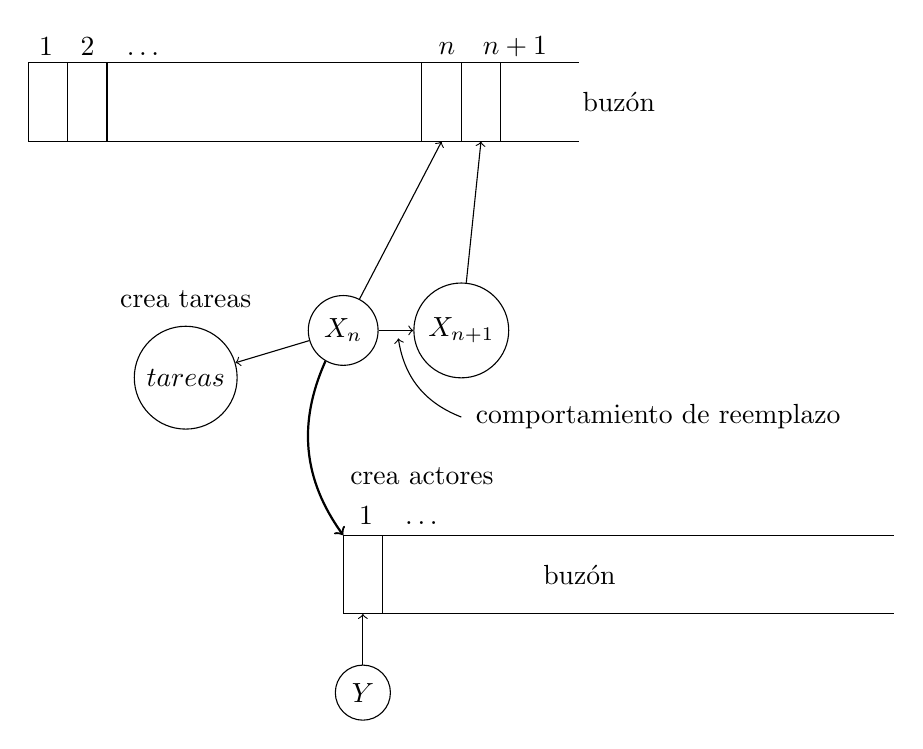
\begin{tikzpicture}

\draw (0,0) -- (7,0);
\draw (0,1) -- (7,1);

\draw (0,0) -- (0,1);
\draw (0.5,0) -- (0.5,1);
\draw (1,0) -- (1,1);

\draw (5,0) -- (5,1);
\draw (5.5,0) -- (5.5,1);
\draw (6,0) -- (6,1);

\node at (0.9,1.2) {$1\quad2\quad\ldots$};

\node at (5.9,1.2) {$n \quad n+1$};

\node at (4,-2.4) [circle,draw] (XN) {$X_n$};
\draw[->] (XN) -- (5.25,0);

\node at (5.5,-2.4) [circle,draw] (XN1) {$X_{n+1}$};
\draw[->] (XN1) -- (5.75,0);

\draw[->] (XN) -- (XN1);

\node at (2,-3) [circle,draw] (T) {$tareas$};

\draw (4,-5) -- (11,-5);
\draw (4,-6) -- (11,-6);
\draw (4,-5) -- (4,-6);
\draw (4.5,-5) -- (4.5,-6);

\draw[->, thick] (XN) to[bend right] (4, -5);

\node at (4.25,-7) [circle,draw] (Y) {$Y$};
\draw[->] (Y) -- (4.25, -6);
\node at (4.70, -4.75) {$1\quad\ldots$};

\draw[->] (XN) -- (T);

\node at (2,-2) {crea tareas};
\node at (5,-4.25) {crea actores};

\node at (8,-3.5) {comportamiento de reemplazo};

\draw[->] (5.5,-3.5) to[bend left] (4.7,-2.5); 

\node at (7.5,0.5) {buzón};
\node at (7,-5.5) {buzón};

\end{tikzpicture}
\caption{Una transición entre dos comportamientos}
\label{fig:actortransition}
\end{figure}

Las dos procesos $X_n$ y $X_{n+1}$ no interfieren entre sí. $X_n$ solo procesa la $(n)-esima$ comunicación. Exceptuando el caso en el cual se envíe una comunicación a si mismo. Cada uno de estos procesos crean sus propias tareas, sus propios actores como esta definido en sus comportamientos. Antes que el proceso $X_n$ cree el proceso $X_{n+1}$, $X_n$ podría haber creado otros actores u otros trabajos. Es posible incluso, que $X_n$ este creando actores o trabajos al mismo tiempo que lo está haciendo $X_{n+1}$. Es importante notar que $X_n$ no recibirá ninguna otra comunicación, ni tampoco especificará ninguno otro comportamiento de reemplazo.

Si definimos que la creación de un actor, la creación de una tarea o especificar el comportamiento de reemplazo son eventos. El orden en que se generan estos eventos debido a que se acepto una comunicación define un orden parcial. El reemplazo de los procesos definen un orden total entre ellos. 

Alguna implementación puede esperar a que el proceso anterior termine, para construir el nuevo y eliminar el viejo. Sin embargo, retrasar el reemplazo hasta que el proceso pueda ser reemplazado no es un requisito. Si hay suficientes recursos disponibles, la computación en un sistema de actores se puede acelerar simplemente aceptando la próxima comunicación ni bien su comportamiento de reemplazo esta establecido.

\begin{figure}[H]
\centering

\tikzstyle{circulo}=[circle,draw=black, fill=black, inner sep=0pt,minimum size=3pt]
\tikzstyle{new}=[-latex, draw, dashed]
\tikzstyle{msg}=[-latex, draw]

\begin{subfigure}{.5\textwidth}
\centering
\begin{tikzpicture}[node distance=2cm]

\node[] (A) {$Actor_1$};
\node[circulo, below of=A] (A1) {};
\node[below of=A1] (A2) {};
\draw (A) -- (A2);

\node[below of=A, right of=A, yshift=1cm] (B) {$Actor_2$};
\node[circulo, below of=A, right of=A] (B1) {};
\node[below of=B1] (B2) {};
\draw (B1) -- (B2);


%\path[msg] (-1/2,-1/2) to [bend right] node[font=\small, left] {$[42]$}  (A1) ;

%\path[new] (A1) to [bend left] node[font=\small, above] {$[7]$} (B1) ;
%\path[new] (A1) to [bend right] node[font=\small, below, pos=0.6] {$[8,9]$} (C1) ;

\path[msg] (-1/2,-1/2) to [bend right] (A1) ;

\path[new] (A1) to [bend left] (B1) ;


\end{tikzpicture}

\caption{  }
\label{fig:actores:crecion:a}
\end{subfigure}%
\begin{subfigure}{.5\textwidth}

\centering
\begin{tikzpicture}[node distance=2cm]

\tikzstyle{circulo}=[circle,draw=black, fill=black, inner sep=0pt,minimum size=3pt]

\node[] (A) {$Actor_1$};
\node[circulo, below of=A] (A1) {};
\node[below of=A1] (A2) {};
\draw (A) -- (A2);

\node[right of=A] (B) {$Actor_2$};
\node[circulo, below of=A, right of=A] (B1) {};
\node[below of=B1] (B2) {};
\draw (B) -- (B2);

\node[right of=B1, yshift=1cm] (C) {$Actor_3$};
\node[circulo, right of=B1] (C1) {};
\node[below of=C1] (C2) {};
\draw (C1) -- (C2);

%\path[msg] (-1/2,-1/2) to [bend right] node[font=\small, left] {$[43]$}  (A1) ;

%\path[msg] (A1) to [bend left] node[font=\small, above] {$[1,2]$} (B1) ;
%\path[new] (B1) to [bend left] node[font=\small, above] {$[3,4]$} (C1) ;

\path[msg] (-1/2,-1/2) to [bend right] (A1) ;
\path[msg] (A1) to [bend left] (B1) ;
\path[new] (B1) to [bend left] (C1) ;

\end{tikzpicture}

\label{fig:actores:crecion:b}
\caption{}
\end{subfigure}

\label{fig:actores:crecion}
\caption{Las lineas verticales indican el paso del tiempo, las de punto indican creación de actores y las otras flechas envío de mensaje.}
\end{figure}

Como se puede ver en la Figura\ref{fig:actores:crecion} \subref{fig:actores:crecion:a}, el actor $Actor_1$ recibe una comunicación con la lista. Al procesar esta comunicación tiene como resultado, crea el actor $Actor_2$. En la Figura\ref{fig:actores:crecion} \subref{fig:actores:crecion:b} se puede ver un ejemplo similar donde $Actor_1$ recibe una comunicación, como resultado envía una comunicación a $Actor_2$ y este último crea $Actor_3$.


\section{Programando con actores}

En esta sección se definirán las construcciones necesarias para definir un núcleo de un lenguaje mínimo de actores. A pesar de su simplicidad, este lenguaje es extremadamente poderoso, captura varias características importantes de la computación dentro del paradigma de actores: la posibilidad de distribuir una computación entre elementos concurrentes, la unificación de información procedural y declarativa, y transparencia referencial de los identificadores usados en un programa.

\subsection{Las construcciones básicas}

En la configuración inicial de un sistema actores, necesitamos crear algunos actores y poderle enviar algunas comunicaciones. Un programa en un sistema de actores esta compuesto por:

\begin{itemize}
 \item \textit{definición de comportamientos} asocia un esquema de comportamiento con un identificador, no crea ningún actor.
 \item expresiones \textit{new} para crear nuevos actores.
 \item comandos \textit{send} para crear nuevas tareas.
\end{itemize}

\subsubsection*{Definiendo comportamientos}\label{actores:comportamientos}
Cada vez que un actor acepta una comunicación, define un comportamiento de reemplazo. Cada uno de los comportamientos de reemplazo también tendrá un comportamiento de reemplazo, para especificar el comportamiento de un actor, necesitamos una definición potencialmente infinita. Para esto acudimos al uso de la reclusión. Básicamente, está parametrizado cada comportamiento mediante algún identificador. Este será una variable libre en la definición del comportamiento. 

Por ejemplo, el comportamiento de una cuenta bancaria depende de su saldo. Entonces se especificará el comportamiento de la cuenta como una función de su saldo. Cada vez que se crea una cuenta, o se define un comportamiento de reemplazo, que usa la definición de comportamiento de una cuenta bancaria, se tiene que dar un valor especifico para esta cuenta.

Podemos concluir que tenemos dos listas de identificadores que son utilizadas en la definición de un comportamiento. La primer lista corresponde a los parámetros que son dados al momento de la creación de un actores. Esta lista es llamada \textit{acquaintance-list}. La segunda lista, que se obtiene cuando una comunicación es aceptada, se llama \textit{communication-list}. Cuando un actor es creado y se acepta una comunicación se ejecutan los comandos en el \textit{entorno} definido por los parámetros enlazados a los identificadores.

\subsubsection*{Creando actores}

Los actores son creados usando expresiones de tipo \textit{new}, que devuelve una nueva dirección de buzón del actor recién creado. La dirección de buzón tiene que estar asignada a algún identificador de caso contrario no tiene ningún sentido, ya que no puede ser utilizada.

La sintaxis de las expresiones de tipo \textit{new} es la siguiente:

\[
   \langle expresi\acute{o}n\ new \rangle :== \textbf{new}\ \langle nombre\ comportamiento \rangle (expr, \{expr\}*)  
\]

$nombre\ comportamiento$ hace referencia a un identificador vinculado con un comportamiento especifico, declarado utilizando una \textit{definición de comportamiento}. Se crea un nuevo actor con el comportamiento descripto en la definición del comportamiento y sus parámetros son instanciados con los valores de las expresiones entre paréntesis. Utilizando el léxico de actores, corresponde a los valores denominados como \textit{acquaintance-list}. El valor de $expresion\ new$ es el valor de la dirección del buzón y está vinculado con un identificador. Este identificador puede ser destino de nuevas comunicaciones. 

Los actores son creados de manera concurrente, estos pueden conocer entre si las dirección de buzón. Esta es una forma de definición mutuamente recursiva que es perfectamente valida en el modelo de actores. En todo actor recientemente creado lo único que el actor que esta creando un nuevo sabe de este es su dirección de buzón, es decir, no tiene ningún acceso a la estructura interna del actor creado.

\subsubsection*{Creando tareas}

Una tarea es creada especificando un actor destino y una comunicación. Las comunicaciones se pueden enviar a actores que ya fueron creados o actores creados por quien está enviando la comunicación. El destino es la dirección de buzón del actor al que le queremos enviar la comunicación. La sintaxis de este comando podría ser la siguiente:

\[
  \langle comando\ send \rangle :== \textbf{send}\ \langle comunicaci\acute{o}n \rangle\ \textbf{to}\ \langle destino \rangle
\]

Donde $comunicaci\acute{o}n$ es una lista de expresiones, que puede ser vacía. Las expresiones pueden ser identificadores, constantes. Las expresiones son evaluadas y se envían los valores en la comunicación. Destino es un identificador que tiene asociado una dirección de buzón de un actor.

\subsubsection*{Comandos}

El propósito de los comandos es especificar las acciones que pueden ocurrir. Se mostraron los comandos para crear nuevos actores y para crear nuevas tareas. También necesitamos un comando para definir el comportamiento de reemplazo. La sintaxis para este comando tiene la forma:

\[
 \texttt{become}\ \langle expresi\acute{o}n \rangle
\]

$expresi\acute{o}n$ debería es una dirección de buzón, entonces este actor reenvía todos los mensajes a el nuevo buzón. También se puede utilizar el identificador de un comportamiento, especificando los parámetros \textit{acquaiantence-list}. Por ejemplo:

\begin{align*}
 \texttt{become}&\ \langle link \rangle \\
 \texttt{become}&\ \langle Comp(1,2,3) \rangle
\end{align*}

Donde $link$ es alguna dirección de buzón, y $Comp(1,2,3)$ hace referencia al comportamiento $Comp$, y su \textit{acquaiantence-list} son los valores $1$, $2$ y $3$.

\section{Lenguaje de Actor Mínimo}\label{actores:sal}

En este capítulo se explorará un lenguaje que implementa los conceptos básicos vistos en la capitulo anterior, tales como comportamientos, creación de nuevos actores, creación de nuevas comunicaciones y otras construcciones. El lenguaje \SAL fue desarrollado con intensiones pedagógicas y tiene una sintaxis heredada de Algol. 

Se utilizará la notación \textbf{Backus-Naur}\cite{McCracken:2003:BF:1074100.1074155} para describir la gramática. Adjunto a la notación se utilizá el símbolo \textbf{*} representa una o ninguna ocurrencias de un termino. También se utilizará \textbf{+} para representar que haya al menos una ocurrencia.

En la última seccione se mostraran dos ejemplos de como se pueden utilizar el lenguaje.

\subsection{Expresiones}\label{actores:exp}
Existen cuatro tipos primitivos, booleanos, enteros, cadenas, y dirección del buzón. Las operaciones posibles entre los booleanos son \textbf{or}, \textbf{and}, \textbf{not}. Los enteros se pueden operar utilizando \textbf{+}, \textbf{-}, \textbf{*}, \textbf{/}. Las cadenas son constantes. La dirección de un buzón es un identificador que es devuelto cuando se crea un nuevo actor, este tipo primitivo no tiene ningún operador asociado.

La gramática de las expresiones booleanas es la siguiente:

\begin{grammar}

<bexp> ::= <bterm> `or' <bterm> | <bterm> `and' <bterm> | <exp> = <exp>
  
<bterm> ::= <bool> | `not' <bterm> | `(' <bexp> `)' 

<bool> ::= `TRUE' | `FALSE'

\end{grammar}

La gramática de los enteros es la siguiente:

\begin{grammar}

<iexp> ::= <iterm> `*' <iterm> | <iterm> `/' <iterm>  
  \alt <iterm> `+' <iterm>  | <iterm> `-' <iterm>

<numero> ::= `1' | `2' | `3' | `4' | `5' | `6' | `7' | `8' | `9' | `0'

<iterm> ::= <numero> "*" | `-' <iterm> | `(' <iexp> `)'

\end{grammar}

La gramática para las cadenas es la siguiente:

\begin{grammar}
 <sexp> ::= `"' <carácter>+ `"'
\end{grammar}

Donde:

\begin{description}
 \item \textit{carácter} es simplemente cualquier carácter entre la $A$ y la $Z$ tanto mayúscula como minúscula
\end{description}

La gramática de todas las expresiones:

\begin{grammar}
<exp> :: = <iexp> | <bexp> | <sexp> | <mexp>  
\end{grammar}

La gramática de $mexp$ es simplemente cualquier carácter entre la $A$ y la $Z$ tanto mayúscula como minúscula. 

\subsection{Definición de comandos}\label{actores:cmd}

% agregar referencia a la seccion de comandos
Los comandos son las acciones que permite a \SAL crear nuevos actores, enviar mensajes y definir un nuevo comportamiento. Estas describen en esencia lo que un actor puede hacer dentro de un comportamiento.

La gramática de los comandos en SAL es la siguiente:

\begin{grammar}
  <command> ::= `send' $exp_1, exp_2, \ldots, exp_n$ `to' <actor>  
  \alt `become' $B(exp_1, exp_2, \ldots, exp_n)$
  \alt `let' $mexp_1$ = `new' $B_1(exp_1, exp_2, \ldots, exp_{1n})$, \\
   \ldots\ \ $mexp_k$ = `new' $B_k(exp_1, exp_2, \ldots, exp_{kn})$   \\
  `in' <command> 
  \alt `if` <bexp> `then' <command> `else' <command> `end if'
  \alt <command> ; <command>
\end{grammar}

donde:

\begin{description}
\item [send] permite enviar mensajes a otros actores, toma como parámetro una lista separada por coma de las expresiones a enviar, y el actor destino. El envío de mensajes es asincrónico. Cada expresión es evaluada antes de ser utilizada como parámetro en \textit{acquaiantence-list}.
\item [become] especifica el siguiente comportamiento del actor que está procesando la comunicación recibida. Como en el caso anterior se evalúan las expresiones antes de utilizadas, y estas aparecerán como la listas de parámetros del comportamiento. 
\item [new] sirve para crear nuevos actores. El alcance de los
  identificadores de los nuevos actores creados está sujeto al cuerpo de \textbf{let}.
\item [if-then-else], después de evaluar la expresión booleana, si es verdadera
  ejecuta lo que esta a continuación de \textbf{then}, en caso contrario lo que está a
  continuación de \textbf{else}. Funciona como cualquier condicional.
\item [composición] Dos comandos que se ejecutan de manera secuencial.

\end{description}

\subsection{Definición de comportamientos}\label{actores:beha}

En esta sección se mostrará la sintaxis para definir comportamientos. Como se vio en el capitulo anterior, la definición de comportamientos tiene asociada dos listas de identificadores, \textit{acquaiantence-list} y \textit{communication-list}. 

En el caso de la lista de identificadores \textit{communication-list}, esta asume que todas las comunicaciones serán una secuencia de identificadores. Supongamos el siguiente caso: un comportamiento que modela una cuenta bancaria. Resulta útil que está lista de identificadores esté dada en función de la operación que se vaya a ejecutar, por ejemplo, si la operación fuera \textit{'extracción'} solamente necesitaríamos un identificador \textit{monto} el cual tendría el valor de la extracción en cuestión. En el caso que la operación fuera \textit{'balance'} esta no requiere identificadores. 

Se presenta a continuación una gramática que contempla el caso en el que solamente necesitemos una lista de identificadores (veremos un ejemplo mas adelante en el ejemplo del calculo del factorial). También se presenta una forma de bifurcarse ante diferentes ramas dependiendo del contenido de la comunicación (el ejemplo que veremos de la una pila hace uso de esto). La gramática de los comportamientos es la siguiente:

\begin{grammar}
<BDef> :== `def' <beh name> `(' <acquaiantence-list> `)' <body> `end def'

<static-list> :== `[`'<comunication-list>`]' \\ <command>*  

<comunication-list> :== <id> | ( <id> `,' <comunication-list> ) *

<match-list> :==  `match' ( `case' `[' <case-list> `]:' <command>* )+  

<case-exp> :== <bool> | <numero> | <id>  

<case-list> :== <case-exp> | ( <case-exp> `,' <case-list> ) *

<acquaiantence-list> :== <id> | ( <id> `,' <acquaiantence-list> ) *

<body> :== <static-list> | <match-list>

\end{grammar}

Donde: 

\begin{description}
 \item \textit{beh name} hace referencia a un comportamiento y tiene alcance a todo el programa. 
 \item \textit{static-list} son completados al momento de procesar una comunicación, y su alcance es todo \textit{command}. 
 \item \textit{comunication-list} se utiliza para definir una lista de identificadores.
 \item \textit{case-exp} puede ser de tipo booleana, un número o un identificador. 
 \item \textit{case-list} se utiliza para definir una lista de elementos de tipo \textit{case-exp}.
 \item \textit{match-list} Se comparan las expresiones una a una, de haber coincidencia se ejecutan los comandos que están a continuación. De contener identificadores libres, estos se inicializarán con el valor contenido en el mensaje para esa posición.
 \item \textit{acquaiantence-list} los recibe al momento de inicialización y tiene alcance en todo \textit{command}.
 \item \textit{body} puede ser una lista de argumentos estática o se puede utilizar el operador \textit{match}.
\end{description}

Podemos pensar que los comportamientos son una función que toma dos listas de parámetros en distintos momentos, uno cuando es inicializada o es invocada desde el cuerpo de un comando utilizando el comando $become$ y el otro conjunto de parámetros los recibe en el momento de procesar un mensaje.

Ambas listas, \textit{comunication-list} y \textit{acquaiantence-list}, contienen todos los identificadores libres que están en \textit{command}. En el caso de \textit{match-list} los identificadores libres tienen alcance a los \textit{commands} asociado a cada \textit{case}. Existe un identificador especial \textit{self} que puede ser utilizado para hacer referencia al buzón del actor que está se definiendo. 

La ejecución de \textit{command} deberá contar a lo sumo con un solo comando \textit{become}, esta propiedad tiene que ser garantizada de manera estática, de no existir ningún comando \textit{become}, el actor asumirá un comportamiento de tipo \textit{bottom}, es es básicamente ignorar los mensajes que se le envíen.

\section{Ejemplos}

En esta sección mostraremos dos ejemplos de \SAL y algunas particularidades del lenguaje. Primero se presentará el código del ejemplo, a continuación una breve descripción linea por linea de la funcionalidad, y para terminar notas sobre su funcionamiento.

\subsection{Cálculo del factorial}\label{sal:factorial}

Se usará este clásico ejemplo, para mostrar que el paso de mensaje se puede usar como una estructura de control. En un lenguaje imperativo una función recursiva está implementada utilizando una Pila de llamadas\footnote{En inglés call stack, \href{https://es.wikipedia.org/wiki/Pila_de_llamadas}{wikipedia}}. Al usar esta pila, implica que factorial solo puede procesar un único calculo a la vez, una vez que termina el calculo puede aceptar nuevamente un calculo. En los lenguajes secuenciales no existe ningún mecanismo que permita distribuir el calculo del factorial o que permita concurrentemente procesar más de una petición.

La implementación depende de crear uno o más trabajadores que están a la espera de la respuesta adecuada. El actor factorial está dispuesto a procesar concurrentemente la próxima comunicación. Esta incluye la dirección de buzón a cual se debe enviar el calculo del factorial.

Está implementación del factorial está adaptada de \cite{Agha:1986:AMC:7929}. Depende de un actor \lstinline[language=sal, style=simple]$Main$ que envía al actor \lstinline[language=sal, style=simple]$Factorial$ el valor a calcular, en el caso del ejemplo el valor $3$. La palabra reservada \textit{self} hace referencia a este buzón, correspondiente al actor que está procesando la comunicación.

Como se verá en el ejemplo, las comunicaciones pueden venir tanto del actor \lstinline[language=sal, style=simple]$Main$ como del actor \lstinline[language=sal, style=simple]$Factorial$.

\begin{lstlisting}[language=sal, style=simple]
def Factorial()[val, customer]
  if val = 0 then
    send [1] to customer
  else
    let cont = new FactorialCont(val, customer)
       in send [val - 1, cont] to self
  end if 
  become Factorial()
end def

def FactorialWorker(n, customer)[m] 
  send [n * m] to customer
end def

def Main() 
  let fact = new Factorial() 
    in send [3, self] to fact
end
\end{lstlisting}

\begin{description}

\item [Linea 1] $Factorial$ no recibe ningún parámetro en el momento de ser inicializado, pero si recibe dos parámetros cuando procesa una comunicación, la lista $[val, customer]$ un entero y una la dirección de un buzón respectivamente.
\item [Linea 2] Asigna como siguiente comportamiento a $Factorial()$, sin parámetros ya que $Factorial$ no recibe ningún parámetro a la inicialización.  
\item [Linea 4] Envía una lista con el valor $1$ al actor con buzón $customer$.
\item [Linea 6] Crea un actor de tipo FactorialWorker. En este caso se utiliza $new$, ya que se está creando un nuevo buzón, y este se asigna a la variable $cont$. Cuando se asigna el nuevo comportamiento, este recibe los parámetros $val$ y $customer$.
\item [Linea 7] Envía un mensaje a la dirección del buzón propio utilizando la palabra reservada $self$, con la lista $val - 1$ y la dirección del buzón que se acaba de crear.
\item [Linea 11] FactorialWorker recibe dos valores cuando es instanciado: un entero $n$ y la dirección de un buzón $customer$. Cuando procesa un mensaje, en su \textit{acquaiantence-list} recibe un entero $m$.
\item [Linea 12] Envía la multiplicación $n*m$ como lista a la dirección del buzón $customer$ 
\item [Lineas 15-18] Inicializa el actor $Factorial$ y le envía a este la lista con los valores $3$ y la dirección del buzón actual. 

\end{description}

Concretamente, el actor ante un entero distinto de cero ejecuta dos acciones, crea un actor que espera un mensaje con un número y multiplicara este numero por \textbf{n} luego se enviará el resultado a el buzón de $customer$.

También, se envía un mensaje a si mismo para evaluar el factorial de \textbf{n - 1}, y como dirección de cliente utiliza la dirección del buzón del actor recientemente creado. Es decir el resultado de $fact(n - 1)$ se le pasará al actor recientemente creado que lo multiplicara por $n$.

Esto establece una red de actores que multiplicaran el valor indicado y enviaran el cálculo al siguiente actor en la red, y el último actor en la red se lo enviará a quien originalmente lo pidió.

En la figura \ref{fig:factorial} se puede ver que el actor $Factorial()$ recibe como comunicación la lista $[3,c]$, esto hace que ocurran dos cosas:

\begin{itemize}
\item Se cree un actor nuevo $FactorialWorker$ con buzón $c1$, este recibe dos parámetros en la inicialización el valor $3$ y el buzón inicial que recibió como comunicación, es decir quien pidió originalmente la computación del factorial de $3$.

\item Se envíe a si mismo el mensaje $[2,c1]$, este inicia el calculo del factorial de $2$, es decir el cálculo de $fact(n-1)$, el paso recursivo.
\end{itemize}

Ahora $c1$ es quien pide el calculo del factorial de $2$. Esto se repite hasta que el valor a calcular es $0$.

Cuando el primer elemento de la comunicación es cero, hace que se le envíe al actor cuya dirección de buzón fue recién recibida, la lista con el valor uno. 

\begin{itemize}
\item $a$ le envía el valor $0$ a $c3$.
\item $c3$ multiplica $1*1$ y se lo envía a $c2$.
\item $c2$ multiplica $2*1$ y se lo envía a $c1$.
\item $c1$ multiplica $3*2$ y se lo envía a $c$.
\end{itemize}

Recordamos que $c$ había pedido el calculo del factorial $3$ en primer lugar.

\begin{figure}[H]
\centering
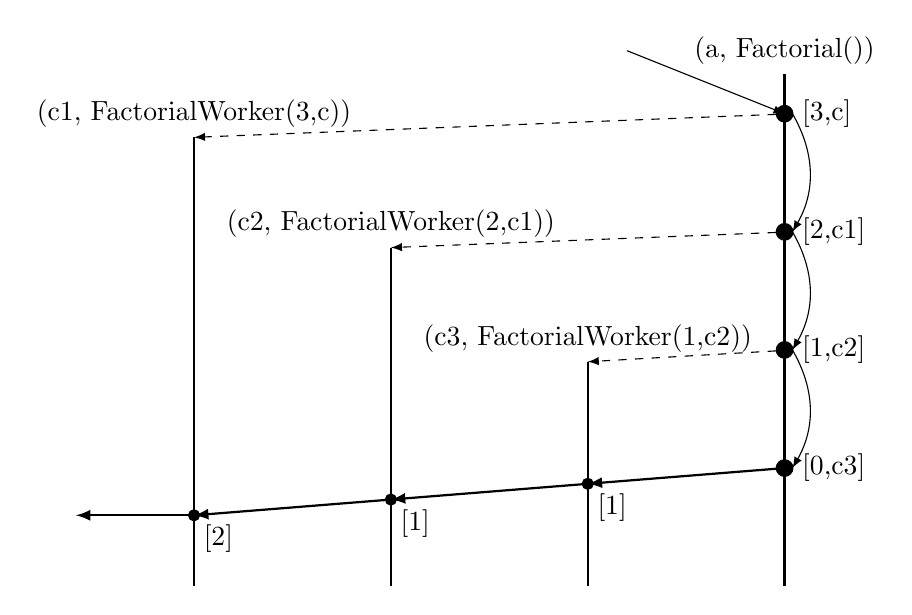
\begin{tikzpicture}

\draw[-latex] (6,7.3) to (8,6.5);

\draw[thick] (8,7) -- (8, 0.5);

\node[] (a1) at (8,7.3) {(a, Factorial())};

\node[align=center, right] (a1) at (8.1,6.5) {[3,c]};
\draw[fill] (8,6.5) circle (3pt);

\node[align=center, right] (a2) at (8.1,5) {[2,c1]};
\draw[fill] (8,5) circle (3pt);

\node[align=center, right] (a3) at (8.1,3.5) {[1,c2]};
\draw[fill] (8,3.5) circle (3pt);

\node[align=center, right] (a4) at (8.1,2) {[0,c3]};
\draw[fill] (8,2) circle (3pt);

\draw[-latex] (a1.west) to[bend left] (a2.west);
\draw[-latex] (a2.west) to[bend left] (a3.west);
\draw[-latex] (a3.west) to[bend left] (a4.west);

\node[] (d1) at (0.5,6.5) {(c1, FactorialWorker(3,c))};
\draw[thick] (d1.south) -- (0.5, 0.5);

\node[] (c1) at (3,5.1) {(c2, FactorialWorker(2,c1))};
\draw[thick] (c1.south) -- (3, 0.5);

\node[] (b1) at (5.5,3.65) {(c3, FactorialWorker(1,c2))};
\draw[thick] (b1.south) -- (5.5, 0.5);

\draw[fill] (5.5,1.8) circle (2pt);
\node[align=center, right] (b2) at (5.5,1.5) {[1]};

\draw[fill] (3,1.6) circle (2pt);
\node[align=center, right] (c2) at (3,1.3) {[1]};

\draw[fill] (0.5,1.4) circle (2pt);
\node[align=center, right] (d2) at (0.5,1.1) {[2]};

\draw[-latex, thick] (8,2)  -- (5.5,1.8);
\draw[-latex, thick] (5.5,1.8) -- (3,1.6);
\draw[-latex, thick] (3,1.6) -- (0.5,1.4);
\draw[-latex, thick] (0.5,1.4) -- (-1,1.4);

\draw[-latex, black, dashed] (a1.west) -- (d1.south);
\draw[-latex, black, dashed] (a2.west) -- (c1.south);
\draw[-latex, black, dashed] (a3.west) -- (b1.south);
\end{tikzpicture}

\caption{El diagrama ilustra el cálculo del factorial de 3, todo el resultado es enviado al actor \textit{c}. Las lineas verticales indican el paso del tiempo, las de punto indican creación de actores y las otras flechas envío de mensaje. La lista superior indica  dirección del buzón, tipo de actor con los parámetros de inicialización.}

\label{fig:factorial}

\end{figure}

\subsection{Una pila usando actores}\label{sal:pila}

Otro ejemplo que podemos encontrar en \cite{Agha:1986:AMC:7929} es el de una pila, que está representada con una lista enlazada. Se utiliza la dirección de un buzón, como un puntero a un nodo de la esta lista. 

Tiene dos operaciones básicas apilar ($push$), que coloca un nodo en la pila, y su operación inversa, sacar ($pop$), que remueve el último elemento agregado en la pila.

\begin{lstlisting}[language=sal, style=simple]
def node(content, link)[operation, customer, newcontent]
  if operation = pop then
    send content to customer;
    become link;
  enf if
  if operation = push then
    let P = new node(content, link)
      in become node(newcontent, P)
  end if
end def

def Main() 
  let stack = new node(10, Nil)
    in send [push, Nil, 20] to stack;
       send [push, Nil, 30] to stack;
  end
end
\end{lstlisting}

\begin{description}

\item [Linea 1] $node$ está inicializado con dos parámetros, $content$ que es un entero, el valor que tiene que guardar el nodo y  $link$ es una dirección de buzón, es el siguiente actor en la pila. Recibe tres parámetros, $operation$ que es el tipo de operación a realizar,  $customer$ que se utiliza cuando la operación es $pop$, y $newcontent$ que se utiliza cuando la operación es $push$.
\item [Linea 3] La instrucción $become$, en este caso, hace que se reenvíen todos los mensajes a la dirección de buzón $link$. 
\item [Linea 4] Envía el contenido del nodo a la dirección de buzón $customer$
\item [Linea 7] Crea un nuevo actor con los parámetros de inicialización $content$ y $link$.
\item [Linea 8] Asigna el siguiente comportamiento, como $node$ con los parámetros $newcontent$ y la dirección de buzón del actor recién creado $P$. 
\item [Lineas 13-15] Crea una nueva pila con uno nodo con valor $10$, y envía dos operaciones $push$ con los valores $20$ y $30$.
\end{description}

El comportamiento $node$ funciona como una lista enlazada, donde en vez de tener direcciones de memoria tenemos direcciones de buzón. El primer parámetro es es el contenido a guardar $content$ y el segundo parámetro $link$ es el actor que está siguiente en la pila, el puntero al siguiente elemento.

Cuando $operation$ es de tipo $pop$, se envía el valor que contiene el nodo al buzón $customer$ y se reenvían todos los mensajes a $link$, todas las futuras operaciones $push$ y $pop$ las recibe este nodo, es decir que ahora es la ``cabeza'' de la pila. Esto guarda un parecido a mover un ``puntero''.

Cuando $operation$ es de tipo $push$, la pila crea un nuevo $node$ que sera el nodo que quedará siguiente en la red, se puede ver que esto ocurre en las lineas 7 y 8. Se copia en $P$ el nodo actual, y crea un nuevo nodo que es la nueva ``cabeza''.

Puede observarse en el ejemplo, que el primer nodo creado tiene como valor $Nil$, esto es simplemente una referencia nula. 

